%==============================================================================
%  STAT 5200 - Applied Econometrics I
%  Homework 1
%
%  Compile with:  pdflatex HW1_report.tex   (run twice for cross-references)
%
%  Directory layout assumed by this file:
%     HW1_report.tex
%     R/q1_matrix_algebra.R
%     R/q1_loop_sum.R
%     R/q2_monte_carlo.R
%     figures/q2_hist_raw.pdf
%     figures/q2_hist_standardised.pdf
%==============================================================================
\documentclass[11pt]{article}

\usepackage[margin=1in]{geometry}
\usepackage[T1]{fontenc}
\usepackage[utf8]{inputenc}
\usepackage{amsmath,amssymb}
\usepackage{booktabs}
\usepackage{graphicx}
\usepackage{xcolor}
\usepackage{listings}
\usepackage[font=small,labelfont=bf]{caption}
\usepackage[hidelinks]{hyperref}

%------------------------------------------------------------------------------
%  Code presentation
%
%  Conventions followed below (standard practice for code in academic reports):
%    * code is set as selectable text in a monospace font, never as a screenshot;
%    * every block is a captioned, labelled float-like object referred to by
%      number in the prose, so the text reads without the code;
%    * source code and program output use visually distinct styles, and are
%      never interleaved in the same block;
%    * only short, load-bearing excerpts appear in the body; the complete
%      scripts are reproduced verbatim in the appendix;
%    * the appendix listings are pulled from the .R files at compile time via
%      \lstinputlisting, so the report cannot drift from the code that was run;
%    * long lines wrap with a visible continuation marker instead of running
%      into the margin.
%------------------------------------------------------------------------------
\definecolor{codekeyword}{RGB}{0,86,148}
\definecolor{codestring} {RGB}{163,21,21}
\definecolor{codecomment}{RGB}{106,115,125}
\definecolor{codebg}     {RGB}{248,248,250}
\definecolor{coderule}   {RGB}{220,220,226}

\lstdefinestyle{Rcode}{
  language        = R,
  basicstyle      = \ttfamily\footnotesize,
  keywordstyle    = \color{codekeyword}\bfseries,
  stringstyle     = \color{codestring},
  commentstyle    = \color{codecomment}\itshape,
  numbers         = left,
  numberstyle     = \ttfamily\scriptsize\color{codecomment},
  numbersep       = 9pt,
  backgroundcolor = \color{codebg},
  frame           = single,
  rulecolor       = \color{coderule},
  framesep        = 4pt,
  xleftmargin     = 20pt,
  xrightmargin    = 2pt,
  breaklines      = true,
  breakatwhitespace = true,
  postbreak       = \mbox{\textcolor{codekeyword}{$\hookrightarrow$}\space},
  showstringspaces = false,
  tabsize         = 2,
  columns         = fullflexible,
  keepspaces      = true,
  captionpos      = b,
  abovecaptionskip = 6pt,
}

% Console output: same monospace face, but unhighlighted and unnumbered, so a
% reader can never mistake output for source.
\lstdefinestyle{Routput}{
  language        = {},          % no keyword highlighting for output
  basicstyle      = \ttfamily\footnotesize,
  keywordstyle    = \ttfamily,
  commentstyle    = \ttfamily,
  stringstyle     = \ttfamily,
  numbers         = none,
  backgroundcolor = \color{white},
  frame           = leftline,
  rulecolor       = \color{coderule},
  framesep        = 6pt,
  xleftmargin     = 20pt,
  breaklines      = true,
  captionpos      = b,
  abovecaptionskip = 6pt,
}

\lstset{style=Rcode}
\renewcommand{\lstlistingname}{Listing}

% Short inline code fragments.
\newcommand{\code}[1]{\texttt{#1}}

%------------------------------------------------------------------------------
\title{\vspace{-2em}Homework 1\\[0.3em]
       \large STAT 5200 --- Applied Econometrics I}
\author{Apostolos Kyratzis - 13130833}
\date{September 17, 2026}

\begin{document}
\maketitle

%==============================================================================
\section{Q1: Basic R questions}
%==============================================================================

\subsection{Matrix algebra}
\label{sec:q1-matrix}

\paragraph{(a) The two matrices.}
We work with
\[
A=\begin{pmatrix} 5 & 2\\ 2 & 1 \end{pmatrix},
\qquad
B=\begin{pmatrix} 5 & 2\\ 2 & 5 \end{pmatrix}.
\]
In R these are built with \code{matrix()}. Because \code{matrix()} fills a
matrix column by column, the argument \code{byrow = TRUE} is used so that the
entries can be typed in the same order in which they are written above; this is
a readability choice, not a mathematical one.

\paragraph{(b) Computing $C = A^{-1}B$.}
Since $\det(A) = 5\cdot 1 - 2\cdot 2 = 1 \neq 0$, the matrix $A$ is invertible,
with
\[
A^{-1} = \frac{1}{\det(A)}\begin{pmatrix} 1 & -2\\ -2 & 5\end{pmatrix}
       = \begin{pmatrix} 1 & -2\\ -2 & 5\end{pmatrix},
\]
so that
\[
C = A^{-1}B
  = \begin{pmatrix} 1 & -2\\ -2 & 5\end{pmatrix}
    \begin{pmatrix} 5 & 2\\ 2 & 5\end{pmatrix}
  = \begin{pmatrix} 1 & -8\\ 0 & 21\end{pmatrix}.
\]
Listing~\ref{lst:q1-core} shows the corresponding R code. Two details are worth
noting. First, \code{solve(A)} returns the inverse of \code{A}, while
\code{\%*\%} performs matrix multiplication. Second, the one-argument form
\code{solve(A)} followed by a multiplication is used here only because the
problem is stated in terms of $A^{-1}$; in applied work the two-argument form
\code{solve(A, B)} is preferred, since it solves the linear system directly and
is both faster and numerically better behaved than forming an explicit inverse.
The script verifies that the two routes agree via \code{all.equal()}.

\begin{lstlisting}[style=Rcode,caption={Constructing $A$ and $B$, and computing
$C=A^{-1}B$ and its transpose (excerpt from \code{R/q1\_matrix\_algebra.R}).},
label={lst:q1-core}]
A <- matrix(c(5, 2,
              2, 1), nrow = 2, ncol = 2, byrow = TRUE)

B <- matrix(c(5, 2,
              2, 5), nrow = 2, ncol = 2, byrow = TRUE)

A_inv <- solve(A)          # solve(A) returns the inverse of A
C     <- A_inv %*% B       # %*% is matrix multiplication

stopifnot(all.equal(C, solve(A, B)))   # same result, better-conditioned route

print(t(C))                # (c) transpose of C
\end{lstlisting}

\paragraph{(c) The transpose of $C$.}
Transposition in R is \code{t()}. The printed result is
\[
C' = \begin{pmatrix} 1 & 0\\ -8 & 21\end{pmatrix},
\]
reproduced as console output below.

\begin{lstlisting}[style=Routput,caption={Console output for
$C$ and $C'$.},label={out:q1-core}]
C = A^{-1} B =
     [,1] [,2]
[1,]    1   -8
[2,]    0   21

t(C) =
     [,1] [,2]
[1,]    1    0
[2,]   -8   21
\end{lstlisting}

\paragraph{(d) The difference between \texttt{A \%*\% B} and \texttt{A * B}.}
The two operators compute genuinely different products.

\code{A \%*\% B} is the \emph{matrix product} of linear algebra. Its $(i,j)$
entry is the inner product of row $i$ of $A$ with column $j$ of $B$,
\[
(A \mathbin{\texttt{\%*\%}} B)_{ij} = \sum_{k} A_{ik} B_{kj},
\]
so it requires the inner dimensions to conform (\code{ncol(A) == nrow(B)}) and
returns an \code{nrow(A)} $\times$ \code{ncol(B)} matrix. It is not commutative.

\code{A * B} is the \emph{element-wise} (Hadamard) product. Its $(i,j)$ entry is
\[
(A \mathbin{\texttt{*}} B)_{ij} = A_{ij} B_{ij},
\]
so it requires the two arrays to have the same shape, returns a matrix of that
same shape, and is commutative. Because \code{*} is an ordinary vectorised
arithmetic operator, it also applies R's recycling rules: \code{A * 2} scales
every entry, and \code{A * c(1, 10)} multiplies the rows of \code{A} by
$1$ and $10$ respectively, because recycling proceeds down columns.

For the matrices in this problem,
\[
A \mathbin{\texttt{\%*\%}} B = \begin{pmatrix} 29 & 20\\ 12 & 9\end{pmatrix},
\qquad
A \mathbin{\texttt{*}} B = \begin{pmatrix} 25 & 4\\ 4 & 5\end{pmatrix}.
\]
The $(1,1)$ entries make the contrast concrete: the matrix product gives
$5\cdot5 + 2\cdot2 = 29$, whereas the element-wise product gives
$5\cdot5 = 25$. Mistaking one for the other is a common and silent bug, since
for square matrices of equal dimension both expressions run without error and
return an object of the same shape.

\subsection{Accumulating a matrix sum with a \texttt{for} loop}
\label{sec:q1-loop}

We compute
\[
X = \sum_{k=1}^{100} D_k,
\qquad
D_k = \begin{pmatrix} k & k+1\\ k^2 & k/2 \end{pmatrix}.
\]
The loop initialises an accumulator at the $2\times2$ zero matrix and adds one
$D_k$ per iteration (Listing~\ref{lst:q1-loop}). Initialising the accumulator
before the loop matters: writing \code{X <- X + D\_k} against an undefined or
\code{NA}-filled \code{X} would either error or propagate \code{NA}s.

\begin{lstlisting}[style=Rcode,caption={Accumulating $X=\sum_{k=1}^{100}D_k$
with a \code{for} loop (excerpt from \code{R/q1\_loop\_sum.R}).},
label={lst:q1-loop}]
K <- 100
X <- matrix(0, nrow = 2, ncol = 2)   # initialise the accumulator

for (k in 1:K) {
  D_k <- matrix(c(k,   k + 1,
                  k^2, k / 2), nrow = 2, ncol = 2, byrow = TRUE)
  X <- X + D_k
}

print(X)
\end{lstlisting}

Because the sum is entry-wise, the answer can be written in closed form using
$\sum_{k=1}^{K}k = K(K+1)/2$ and $\sum_{k=1}^{K}k^2 = K(K+1)(2K+1)/6$. With
$K=100$,
\[
X =
\begin{pmatrix}
\sum k & \sum (k+1)\\[2pt]
\sum k^2 & \sum k/2
\end{pmatrix}
=
\begin{pmatrix}
5050 & 5150\\
338{,}350 & 2525
\end{pmatrix}.
\]
The script computes this closed form and checks it against the loop result with
\code{stopifnot(all.equal(X, X\_closed))}; the check passes, which is reported in
the output below. Verifying a loop against an independent closed-form expression
is cheap here and is good practice generally.

\begin{lstlisting}[style=Routput,caption={Console output for
$X=\sum_{k=1}^{100}D_k$.},label={out:q1-loop}]
X = sum_{k=1}^{100} D_k =
       [,1] [,2]
[1,]   5050 5150
[2,] 338350 2525

Loop and closed-form results agree.
\end{lstlisting}

%==============================================================================
\section{Q2: Monte Carlo simulation (Lab Notes 01 quiz)}
\label{sec:q2}
%==============================================================================

\subsection{Setup}

The population model is
\[
y = \beta_0 + \beta_1 x + \beta_2 x^2 + \varepsilon,
\qquad
\beta_0 = 1,\; \beta_1 = 1,\; \beta_2 = 0.2,
\qquad
x \sim N(1, 4),
\]
and the object of interest is $\theta_0 = E[y]$, estimated by the sample mean
$\hat\theta = N^{-1}\sum_{i=1}^{N} y_i$.

The quiz replaces the original error distribution $\varepsilon \sim t_{10}$ with
\[
\varepsilon = v - 20, \qquad v \sim \chi^2(20).
\]
Both specifications have mean zero, since $E[v] = 20$. The population object of
interest is therefore unchanged:
\[
\theta_0 = E[y] = \beta_0 + \beta_1 E[x] + \beta_2 E[x^2] + E[\varepsilon]
        = 1 + 1 + 0.2 \times 5 = 3 .
\]
What does change is the error variance, and this is the key to the whole
exercise: $\operatorname{Var}(t_{10}) = 10/8 = 1.25$, whereas
$\operatorname{Var}(\chi^2(20)) = 2 \times 20 = 40$. The new errors are also
right-skewed rather than symmetric.

Since $\hat\theta$ is the mean of $N$ i.i.d.\ draws of $y$, we have
$\operatorname{Var}(\sqrt{N}\hat\theta) = N \operatorname{Var}(\hat\theta)
= \operatorname{Var}(y)$ exactly, for every $N$. For $x \sim N(1,4)$ one obtains
$\operatorname{Var}(x) = 4$, $\operatorname{Var}(x^2) = 48$ and
$\operatorname{Cov}(x, x^2) = 8$, hence
\[
\operatorname{Var}(\beta_1 x + \beta_2 x^2)
 = 4 + 0.2^2 \times 48 + 2 \times 0.2 \times 8 = 9.12,
\]
and so $\operatorname{Var}(y) = 9.12 + \operatorname{Var}(\varepsilon)$, giving
$10.37$ under the $t_{10}$ errors and $49.12$ under the $\chi^2$ errors. These
two numbers are the benchmarks against which the simulation is read.

\subsection{Implementation}

Rather than duplicating the lab code, the data generating process takes the
error specification as an argument, so that the original and the quiz model run
through identical code paths (Listing~\ref{lst:q2-dgp}). This removes the
possibility that a difference in results is an artefact of a difference in
implementation.

\begin{lstlisting}[style=Rcode,caption={The data generating process, with the
error distribution as an argument (excerpt from \code{R/q2\_monte\_carlo.R}).},
label={lst:q2-dgp}]
draw_error <- function(error = c("t10", "chi2")) {
  error <- match.arg(error)
  if (error == "t10") {
    rt(1, df = 10)               # eps ~ t(10)
  } else {
    rchisq(1, df = 20) - 20      # eps = v - 20, v ~ chi^2(20)
  }
}

generate_data <- function(N = 20, error = c("t10", "chi2")) {
  error <- match.arg(error)
  mat_data <- matrix(NA, N, 2)   # N by 2 matrix to store (y, x) by row
  for (i in 1:N) {
    e <- draw_error(error)
    x <- rnorm(1, mean = x_mean, sd = sqrt(x_var))
    y <- beta0 + beta1 * x + beta2 * x^2 + e
    mat_data[i, ] <- c(y, x)
  }
  colnames(mat_data) <- c("y", "x")
  return(mat_data)
}
\end{lstlisting}

The Monte Carlo loop itself is unchanged from the lab notes: for a given $N$ it
generates $M = 1000$ data sets, computes the sample mean of $y$ in each, and
returns the $M$ estimates (Listing~\ref{lst:q2-mc}). The experiment is then run
on the grid $N \in \{20, 100, 500\}$ for both error specifications.

\begin{lstlisting}[style=Rcode,caption={The Monte Carlo loop (excerpt from
\code{R/q2\_monte\_carlo.R}).},label={lst:q2-mc}]
simulation_sample_mean <- function(N = 20, M = 1000, error = c("t10", "chi2")) {
  error <- match.arg(error)
  mat_theta_hat <- matrix(NA, M, 1)   # placeholder for the M sample means
  for (m in 1:M) {
    dataset            <- generate_data(N, error)
    mat_theta_hat[m, ] <- mean(dataset[, "y"])
  }
  return(mat_theta_hat)
}
\end{lstlisting}

\subsection{Results}

Table~\ref{tab:q2} collects the Monte Carlo results.

\begin{table}[htbp]
\centering
\caption{Monte Carlo properties of the sample mean, $M = 1000$ replications,
$\theta_0 = 3$. The last column should be compared with
$\operatorname{Var}(y)$, which equals $10.37$ under $t_{10}$ errors and
$49.12$ under $\chi^2$ errors.}
\label{tab:q2}
\small
\begin{tabular}{llccc}
\toprule
Error specification & $N$ & mean$(\hat\theta)$ &
$\operatorname{Var}(\hat\theta)$ &
$\operatorname{Var}(\sqrt{N}\hat\theta)$ \\
\midrule
$\varepsilon \sim t_{10}$ (original)
  & 20  & 2.966 & 0.4982 & \phantom{0}9.963 \\
  & 100 & 2.988 & 0.0989 & \phantom{0}9.892 \\
  & 500 & 3.000 & 0.0200 & 10.016 \\
\addlinespace
$\varepsilon = v - 20$, $v \sim \chi^2(20)$ (quiz)
  & 20  & 3.040 & 2.4771 & 49.541 \\
  & 100 & 3.001 & 0.4786 & 47.859 \\
  & 500 & 2.992 & 0.1024 & 51.181 \\
\bottomrule
\end{tabular}
\end{table}

\paragraph{Do we reach the same conclusion under the new population model?}
Yes --- every qualitative conclusion of the lab notes carries over, and only the
scale of the sampling uncertainty changes.

\begin{enumerate}
\item \emph{The estimator remains centred on $\theta_0 = 3$.} The Monte Carlo
means are $3.040$, $3.001$ and $2.992$, consistent with $\hat\theta$ being
unbiased. This is expected, because recentring the $\chi^2(20)$ draws at
$v - 20$ preserves $E[\varepsilon] = 0$ and hence leaves $E[y] = 3$ intact.

\item \emph{$\operatorname{Var}(\hat\theta)$ still falls at rate $1/N$.} Moving
from $N = 20$ to $N = 100$ divides the variance by $2.4771 / 0.4786 = 5.18$, and
moving from $N = 100$ to $N = 500$ divides it by $0.4786 / 0.1024 = 4.67$. Both
are close to the factor of $5$ by which $N$ was increased; the departures are
Monte Carlo noise from using only $M = 1000$ replications.

\item \emph{$\operatorname{Var}(\sqrt{N}\hat\theta)$ is stable in $N$.} The
values $49.54$, $47.86$ and $51.18$ show no trend and sit around the theoretical
$\operatorname{Var}(y) = 49.12$. The $\sqrt{N}$ scaling is exactly the rate that
offsets the $1/N$ shrinkage, which is why this quantity has a non-degenerate
limit and why $\sqrt{N}$ is the natural normalisation in asymptotic theory.
\end{enumerate}

The one substantive difference is the \emph{level}: sampling uncertainty is
roughly $49.12 / 10.37 \approx 4.7$ times larger under the new model, because
$\operatorname{Var}(\varepsilon)$ rises from $1.25$ to $40$ while the
contribution of $x$ stays at $9.12$. A noisier population requires a larger
sample to attain the same precision --- to match the precision that the original
model achieves at $N = 100$, the new model needs roughly $N = 470$. So the
conclusions about the \emph{rates} are unchanged; what changes is how much data
is needed in practice.

\paragraph{Histograms of $\sqrt{N}\hat\theta$ at $N = 500$.}
Figure~\ref{fig:q2-raw} plots the two simulated distributions on a common
horizontal axis. Both are single-peaked, symmetric and centred on
$\sqrt{500} \times 3 \approx 67.08$, but the $\chi^2$ case is visibly wider,
which is the variance difference of Table~\ref{tab:q2} seen directly.

\begin{figure}[htbp]
\centering
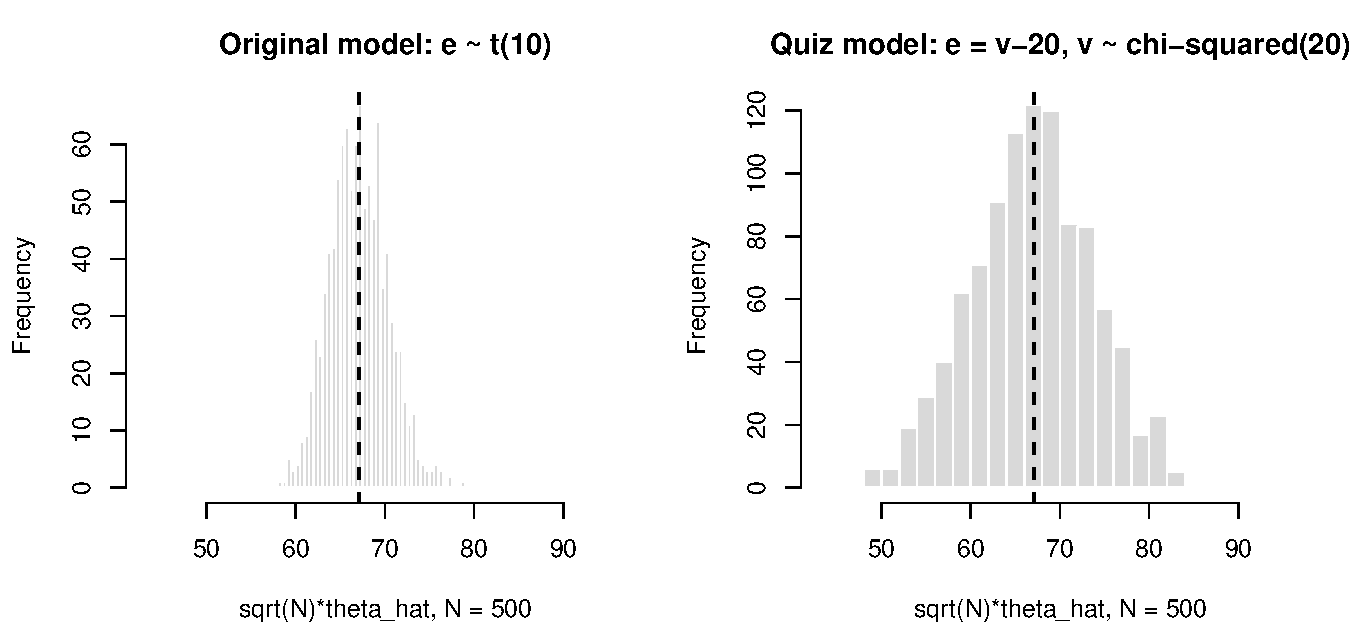
\includegraphics[width=\textwidth]{figures/q2_hist_raw.pdf}
\caption{Simulated distribution of $\sqrt{N}\hat\theta$ at $N = 500$,
$M = 1000$, on a common horizontal axis. The dashed line marks
$\sqrt{N}\theta_0 \approx 67.08$. Left: original $t_{10}$ errors. Right: the
quiz model, $\varepsilon = v - 20$ with $v \sim \chi^2(20)$.}
\label{fig:q2-raw}
\end{figure}

To compare the \emph{shapes} rather than the scales, Figure~\ref{fig:q2-std}
standardises each set of draws and overlays the standard normal density. The two
histograms are then nearly indistinguishable, and both track the normal curve
closely.

\begin{figure}[htbp]
\centering
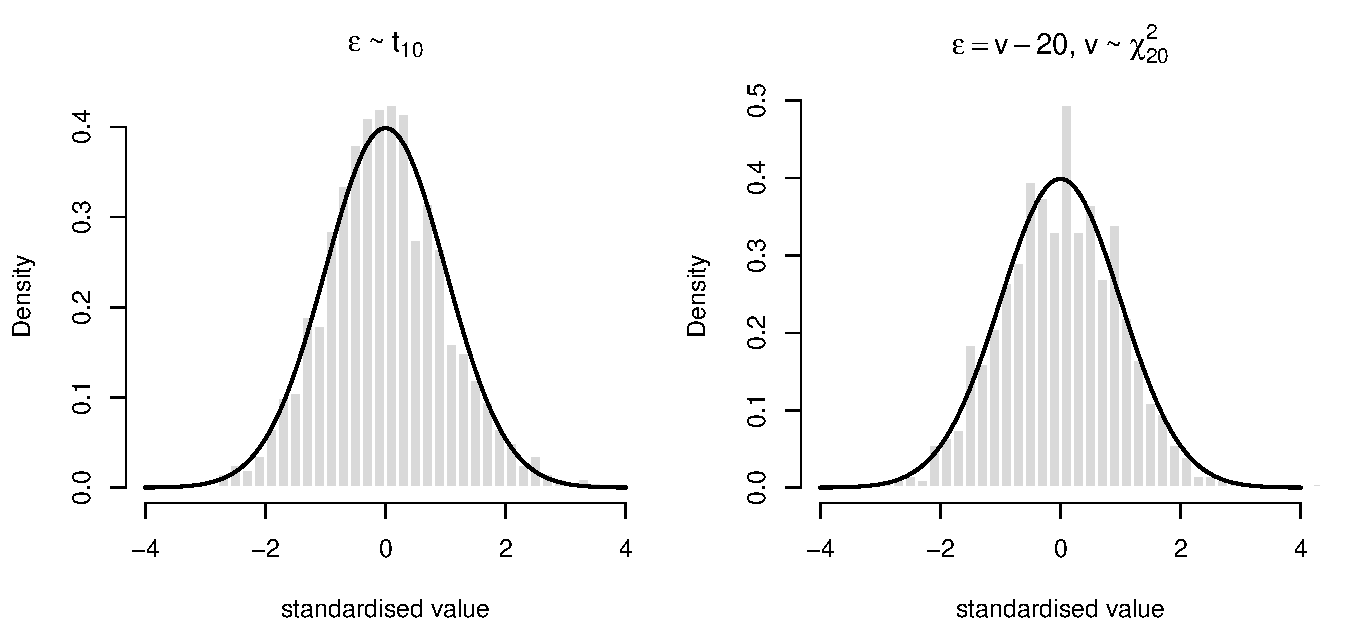
\includegraphics[width=\textwidth]{figures/q2_hist_standardised.pdf}
\caption{The same draws as Figure~\ref{fig:q2-raw}, standardised to mean zero
and unit variance, with the standard normal density overlaid. Once the
difference in scale is removed, the two sampling distributions have essentially
the same shape.}
\label{fig:q2-std}
\end{figure}

So the answer is: \emph{yes, they look similar} --- and the reason is the central
limit theorem rather than any similarity between the two error distributions
themselves. A $\chi^2(20)$ variable is right-skewed, so individual observations
$y_i$ are skewed in a way they are not under symmetric $t_{10}$ errors. But
$\hat\theta$ averages $N = 500$ of them, and the CLT implies
\[
\sqrt{N}\,(\hat\theta - \theta_0) \;\xrightarrow{d}\;
N\!\left(0, \operatorname{Var}(y)\right),
\]
which requires only a finite variance, not normality or symmetry of the
underlying draws. The skewness of the individual observations is averaged away:
the measured skewness of $\sqrt{N}\hat\theta$ at $N = 500$ is $0.10$ in the
$\chi^2$ case and $0.21$ in the $t_{10}$ case, both effectively zero at
$M = 1000$. The limiting distributions therefore differ only through the
variance $\operatorname{Var}(y)$ --- which is exactly the parameter that
Figure~\ref{fig:q2-raw} displays and that Figure~\ref{fig:q2-std} removes.

%==============================================================================
\section{Q3: Paper questions}
%==============================================================================

\emph{To be completed.}

\begin{enumerate}
\item Field of interest.
\item Five well-read journals in the field.
\item The paper found, satisfying the four stated criteria.
\item Full citation.
\item The main research question, in one paragraph.
\item The econometric method used.
\item Whether standard errors are reported.
\item (Not graded) What a standard error is.
\end{enumerate}

%==============================================================================
\appendix
\section{Complete R scripts}
\label{app:code}
%==============================================================================

The listings in this appendix are read directly from the \code{.R} files at
compile time, so they are verbatim copies of the code that produced the results
above.

\subsection{\texorpdfstring{\code{R/q1\_matrix\_algebra.R}}{R/q1\_matrix\_algebra.R}}
\lstinputlisting[style=Rcode,caption={\code{R/q1\_matrix\_algebra.R} --- Q1.2,
matrix algebra.},label={lst:app-q1a}]{R/q1_matrix_algebra.R}

\subsection{\texorpdfstring{\code{R/q1\_loop\_sum.R}}{R/q1\_loop\_sum.R}}
\lstinputlisting[style=Rcode,caption={\code{R/q1\_loop\_sum.R} --- Q1.3, matrix
sum accumulated with a \code{for} loop.},label={lst:app-q1b}]{R/q1_loop_sum.R}

\subsection{\texorpdfstring{\code{R/q2\_monte\_carlo.R}}{R/q2\_monte\_carlo.R}}
\lstinputlisting[style=Rcode,caption={\code{R/q2\_monte\_carlo.R} --- Q2, Monte
Carlo study of the sample mean under both error
specifications.},label={lst:app-q2}]{R/q2_monte_carlo.R}

\end{document}
